\subsection{Diseño Tridimensional del Armazón}

\par
Para el Diseño del armazón debemos crear un modelo digital de las medidas del prototipo, específicamente un modelo de la figura 4.30. En el programa fusion 360 el modelo sería el siguiente.

\begin{figure}[H]
	\centering
	\includegraphics[width=0.8\linewidth]{armazon00.png}
	\caption{Diseño Digital del prototipo (pantalla y circuito impreso)}
\end{figure}

\par \noindent
En la imagen 4.31 se pude apreciar el diseño de la pantalla de color rojo, el circuito impreso o placa en verde y podemos observar ciertos elementos de color negro. Dos de ellos sobresalen de la placa del prototipo; el cilíndrico vendría siendo la conexión del sensor de temperatura, jack de 3.5 mm y uno rectangular el cual sería el switch para encender o apagar el prototipo. Esto es muy importante que se encuentre en el modelo debido a que el armazón estará compuesto de dos moldes.  

\par \noindent
Un molde superior que cubrirá la pantalla y un molde inferior que cubrirá el resto del prototipo. Ambos moldes deben encapsular el prototipo, tener las mismas dimensiones y debe contar con un mecanismo para que el armazón no se separe en caso de una caída por el usuario.

\subsubsection{Molde Superior}

\par 
El molde superior es la presentación del prototipo es donde solamente se debe ver la pantalla LCD. A su vez si observamos las imágenes 4.29 y 4.31, la pantalla LCD no es completamente plana. Posee ciertas dimensiones de altura que debemos tomar en cuenta. 

\par \noindent
Una regla general que vamos a adoptar es que los moldes del armazón deben contar con un borde de menos de 2mm. Esto es para brindarle al armazón una base solida y una protección al prototipo. Lo primero que debemos de hacer es dibujos en plano del molde y todas sus partes.

\begin{figure}[H]
	\centering
	\includegraphics[width=0.5\linewidth]{armazon01.png}
	\caption{Dibujo del Area del Molde Superior}
\end{figure}

\begin{figure}[H]
	\centering
	\includegraphics[width=0.5\linewidth]{armazon04.png}
	\caption{Dibujo detallado de la pantalla LCD}
\end{figure}

\begin{figure}[H]
	\centering
	\includegraphics[width=0.6\linewidth]{armazon02.png}
	\caption{Dibujo del Area y bordes del circuito impreso o placa}
\end{figure}

\begin{figure}[H]
	\centering
	\includegraphics[width=0.6\linewidth]{armazon03.png}
	\caption{Dibujo de circunferencias para el uso de tornillos en el molde}
\end{figure}

\clearpage

\par \noindent
Ahora que tenemos definidos los dibujos procedemos a diseñar el molde superior.

\begin{figure}[H]
	\centering
	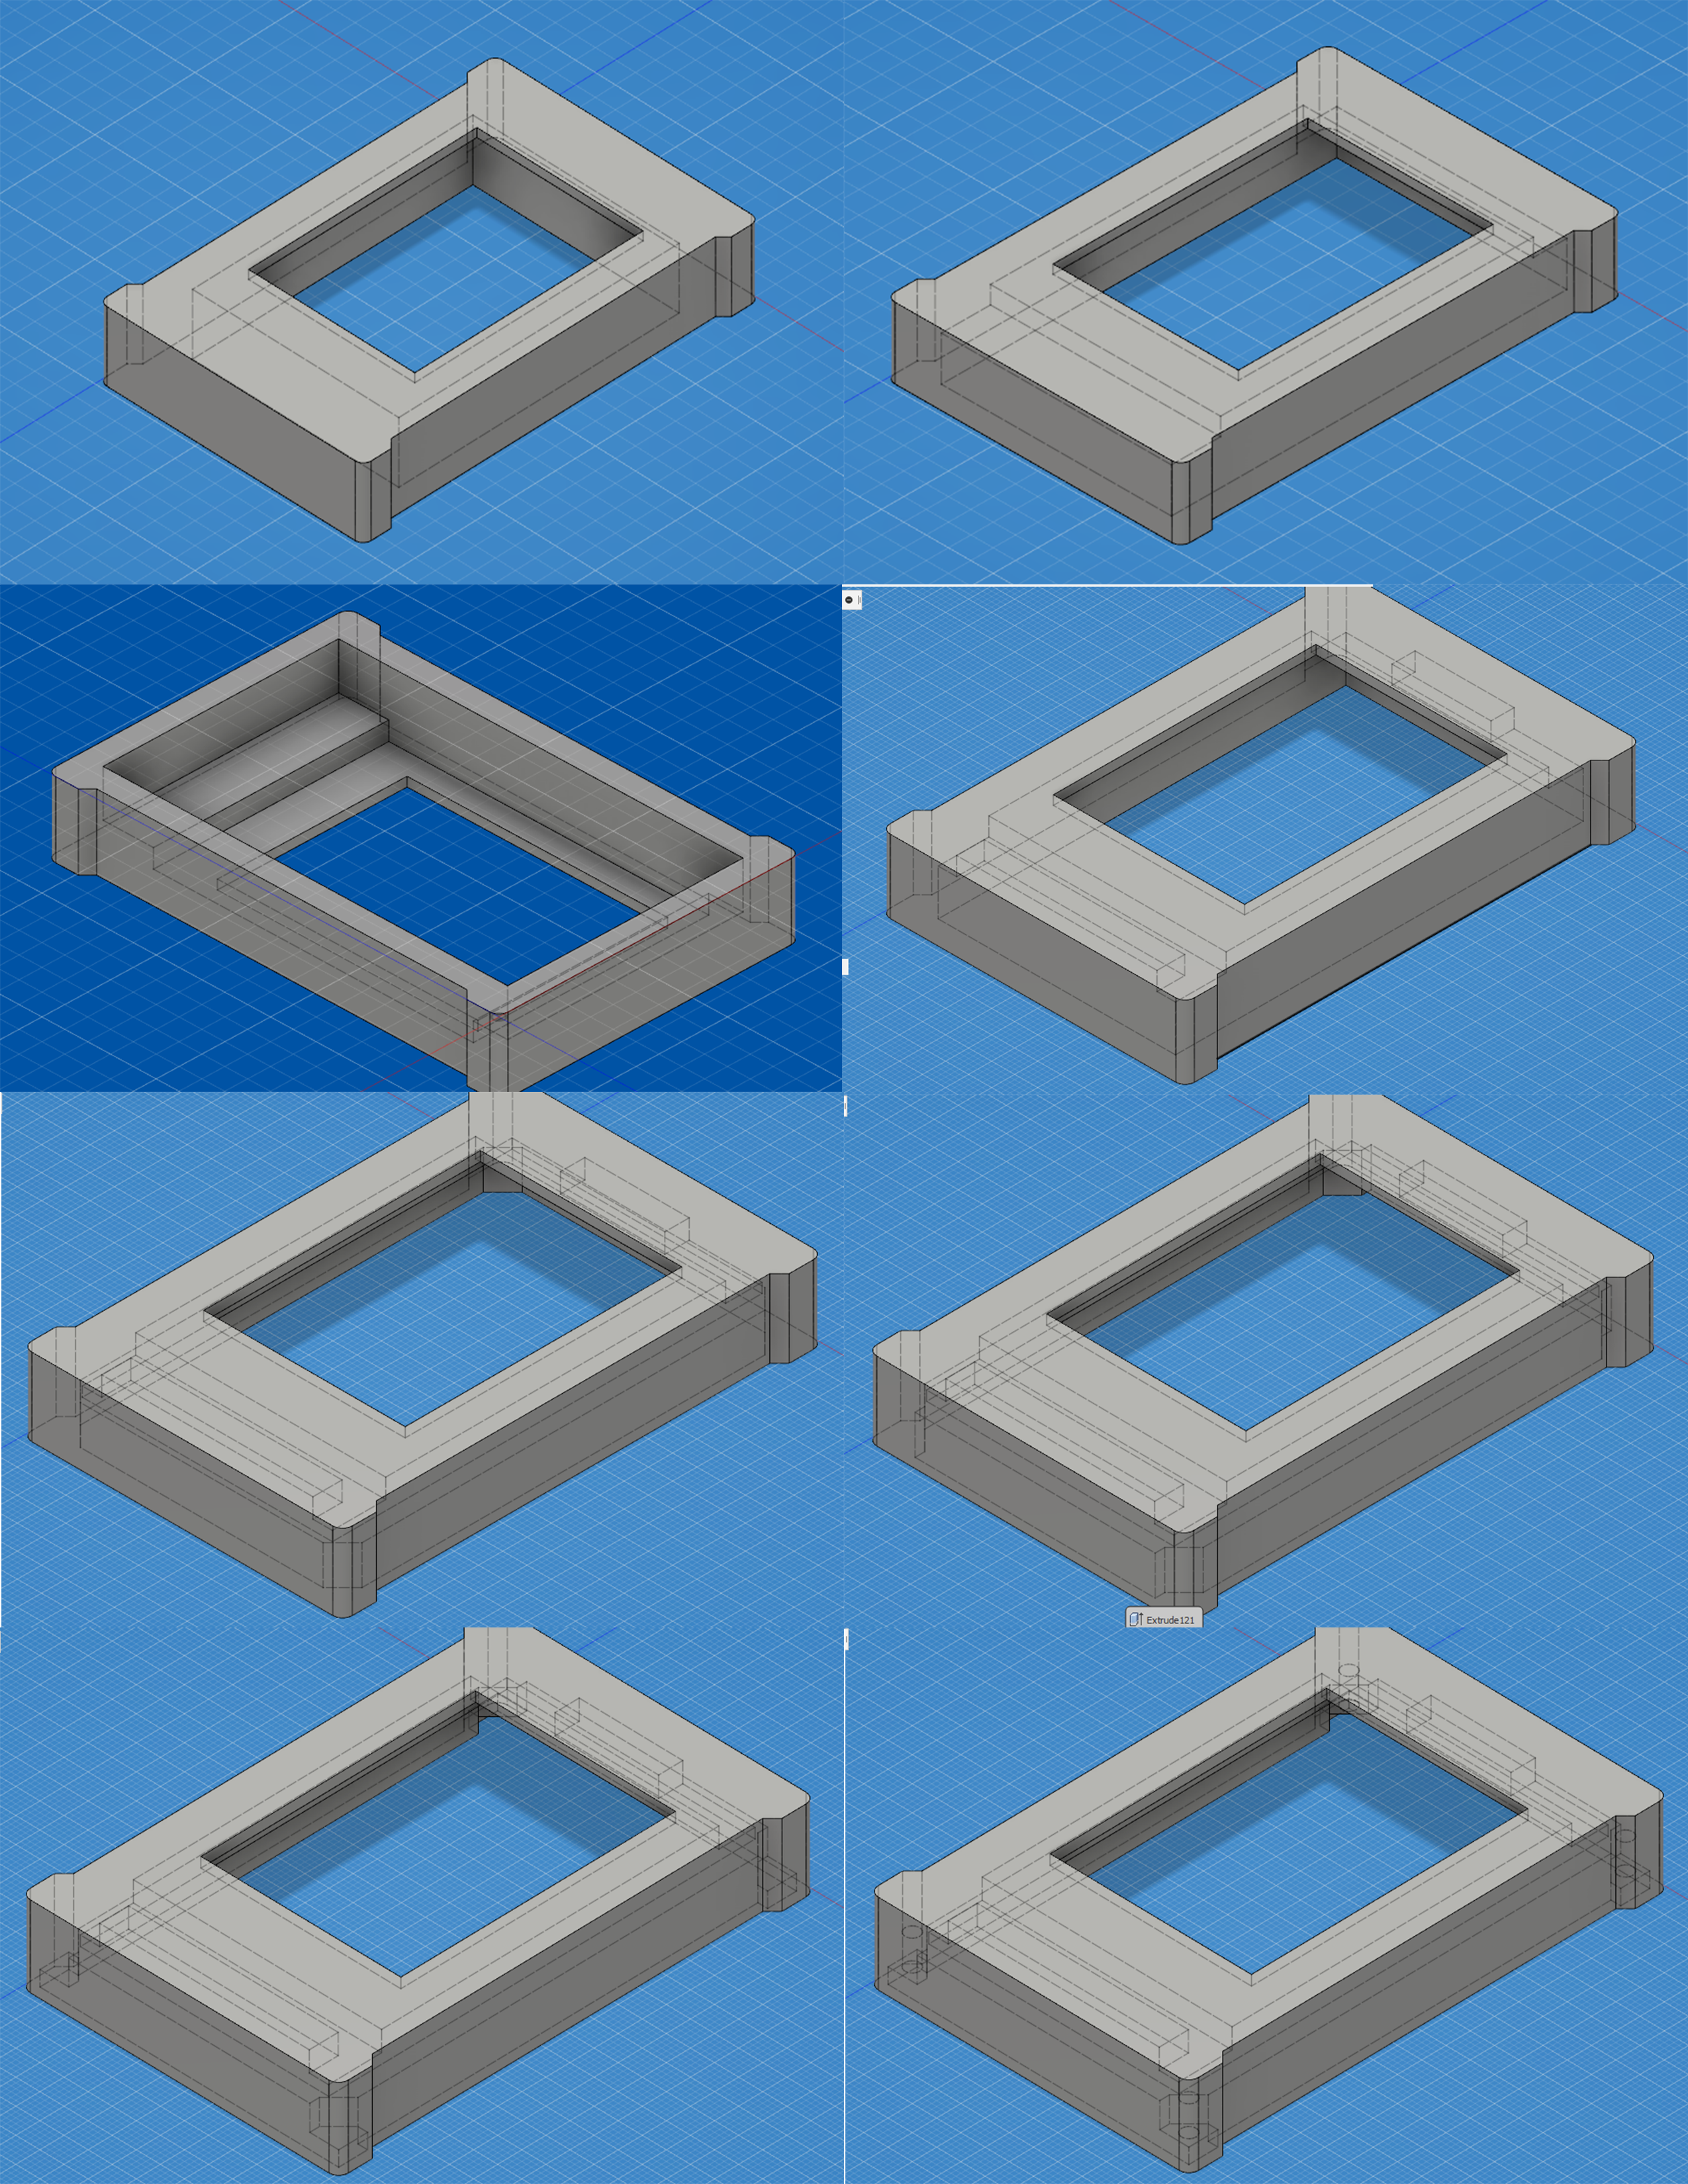
\includegraphics[width=0.8\linewidth]{armazon05.png}
	\caption{Proceso del Diseño del Molde Superior Parte 1}
\end{figure}

\par \noindent
En la figura 4.36 se puede ver como se inicia el diseño del armazón. El diseño del molde superior empieza extrudiendo del dibujo de la figura 4.32; subimos el dibujo unos 17 mm y creamos el orificio donde se vera la pantalla LCD. A partir de allí se empieza a modelar la entrada para la pantalla LCD y el espacio para la placa del prototipo. Una vez diseñado eso en las esquinas se deja un espacio diagonal; específicamente como en la figura 4.34, estos espacios tendrán 3 mm de diferencia con el resto del molde esto es para insertar el molde inferior. Adicional se agregar los orificios donde modelaremos la entrada de tornillos.

\begin{figure}[H]
	\centering
	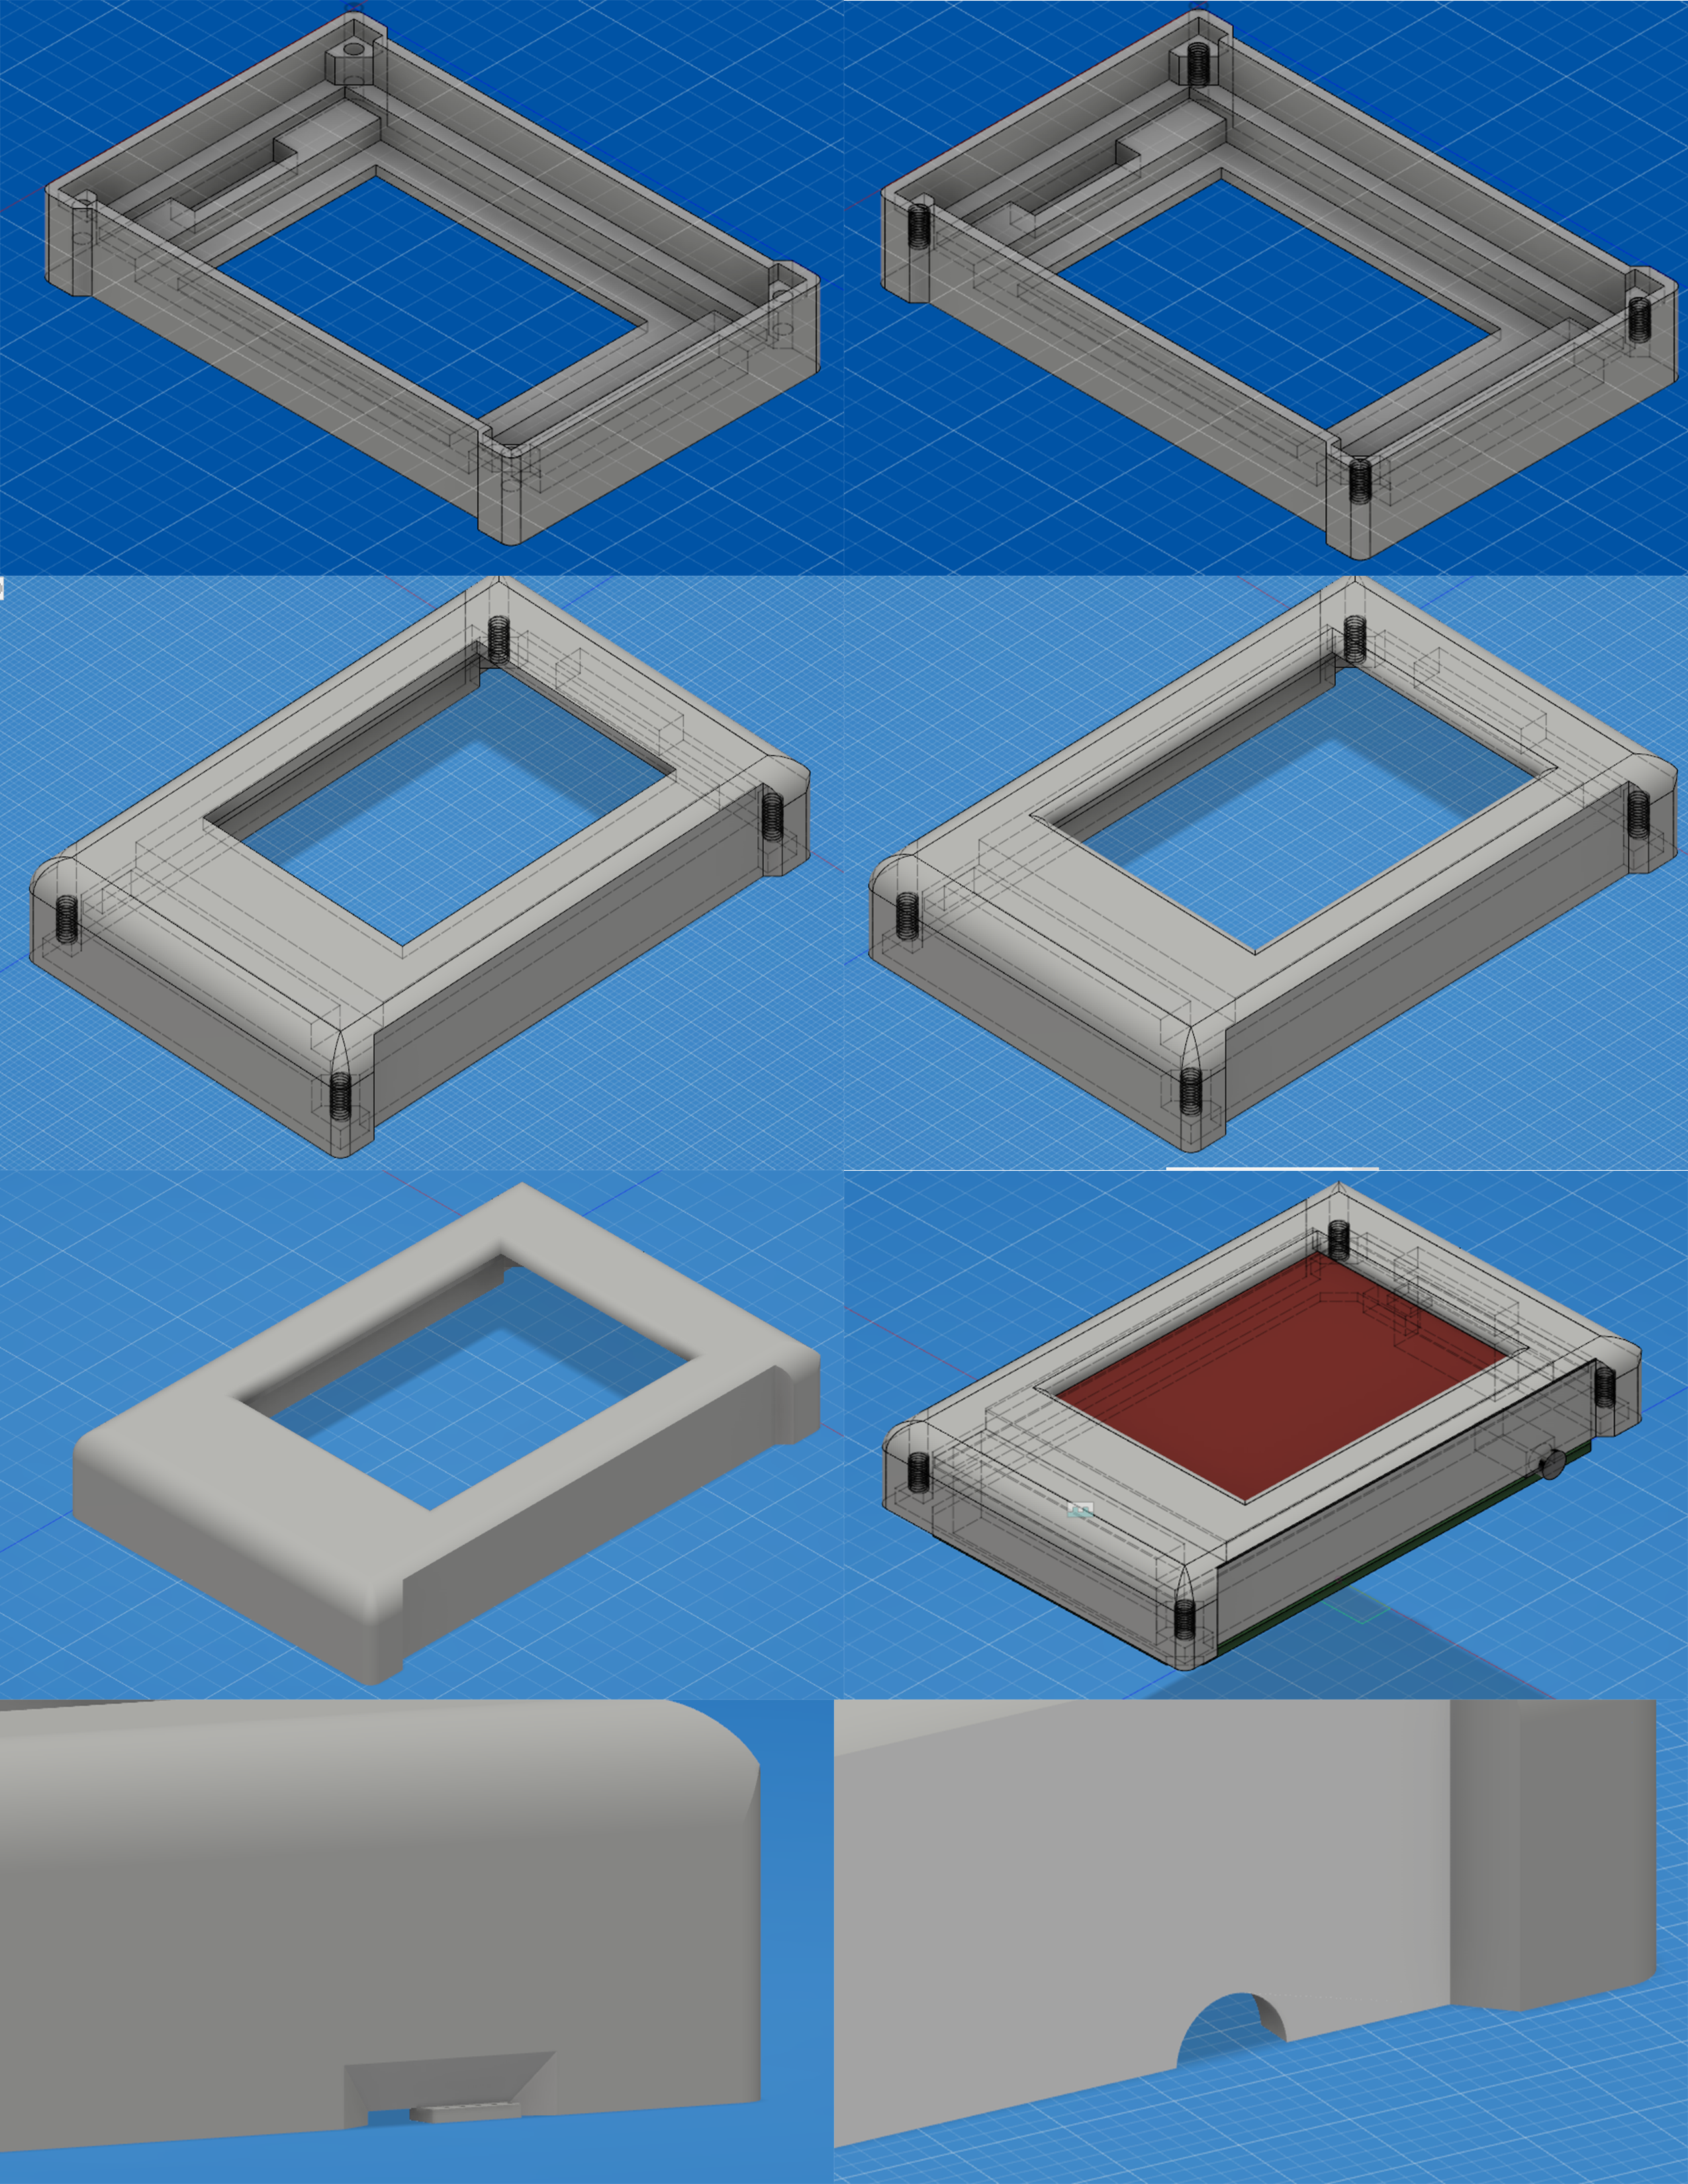
\includegraphics[width=0.8\linewidth]{armazon06.png}
	\caption{Proceso del Diseño del Molde Superior Parte 1}
\end{figure}

\par \noindent
En la figura 4.37 al inicio podemos apreciar todo lo que se realizo en la figura 4.36. Todo esto es para que la pantalla LCD entre sin problemas en el molde. Seguido modelamos las entradas para tornillos en los orificios de las esquinas. Los tornillos para los que estamos modelando son para tornillos de calibre M3. Una vez realizado eso redondeamos los bordes frontales del molde para darle un aspecto mas profesional y por ultimo cortamos los espacios para la entrada del sensor de temperatura y el interruptor para encender el prototipo. El resultado final es el siguiente.

\begin{figure}[H]
	\centering
	\includegraphics[width=0.8\linewidth]{armazon07.png}
	\caption{Diseño del molde superior finalizado}
\end{figure}

\par \noindent
Finalizado el diseño del molde superior procedemos a diseñar el molde inferior.

\subsubsection{Molde Inferior}

\par \noindent
El molde inferior es donde se encontrara la batería de nuestro dispositivo y debe unirse al molde superior y deberá contar con un espacio para que tornillos puedan mantener unido ambos moldes sin problemas. El molde sera basado en los mismos dibujos utilizados por el molde superior. 

\par \noindent
El molde inferior tiene una particularidad y es que debemos tener un espacio para un modulo de carga de la batería por lo que es necesario un corte para la entrada de micro-usb. 

\par \noindent
Observando la imagen 4.38 hay un corte de una circunferencia por donde se conectara el sensor de temperatura. El corte es a la mitad de la circunferencia para una inserción del prototipo al armazón mas sencilla. Adicional hay un espacio en la parte superior del armazón para el interruptor de encendido del prototipo que también se encuentra a la mitad. Ambos cortes debemos tenerlos presentes para el molde inferior. Para mantener la placa sin contacto directo con la batería y tener los cortes necesarios para las entradas del prototipo debemos colocar unos pequeños brazos para que la placa del prototipo tenga donde sostenerse.

\begin{figure}[H]
	\centering
	\includegraphics[width=0.7\linewidth]{armazon08.png}
	\caption{Proceso del diseño del molde inferior parte 1}
\end{figure}

\begin{figure}[H]
	\centering
	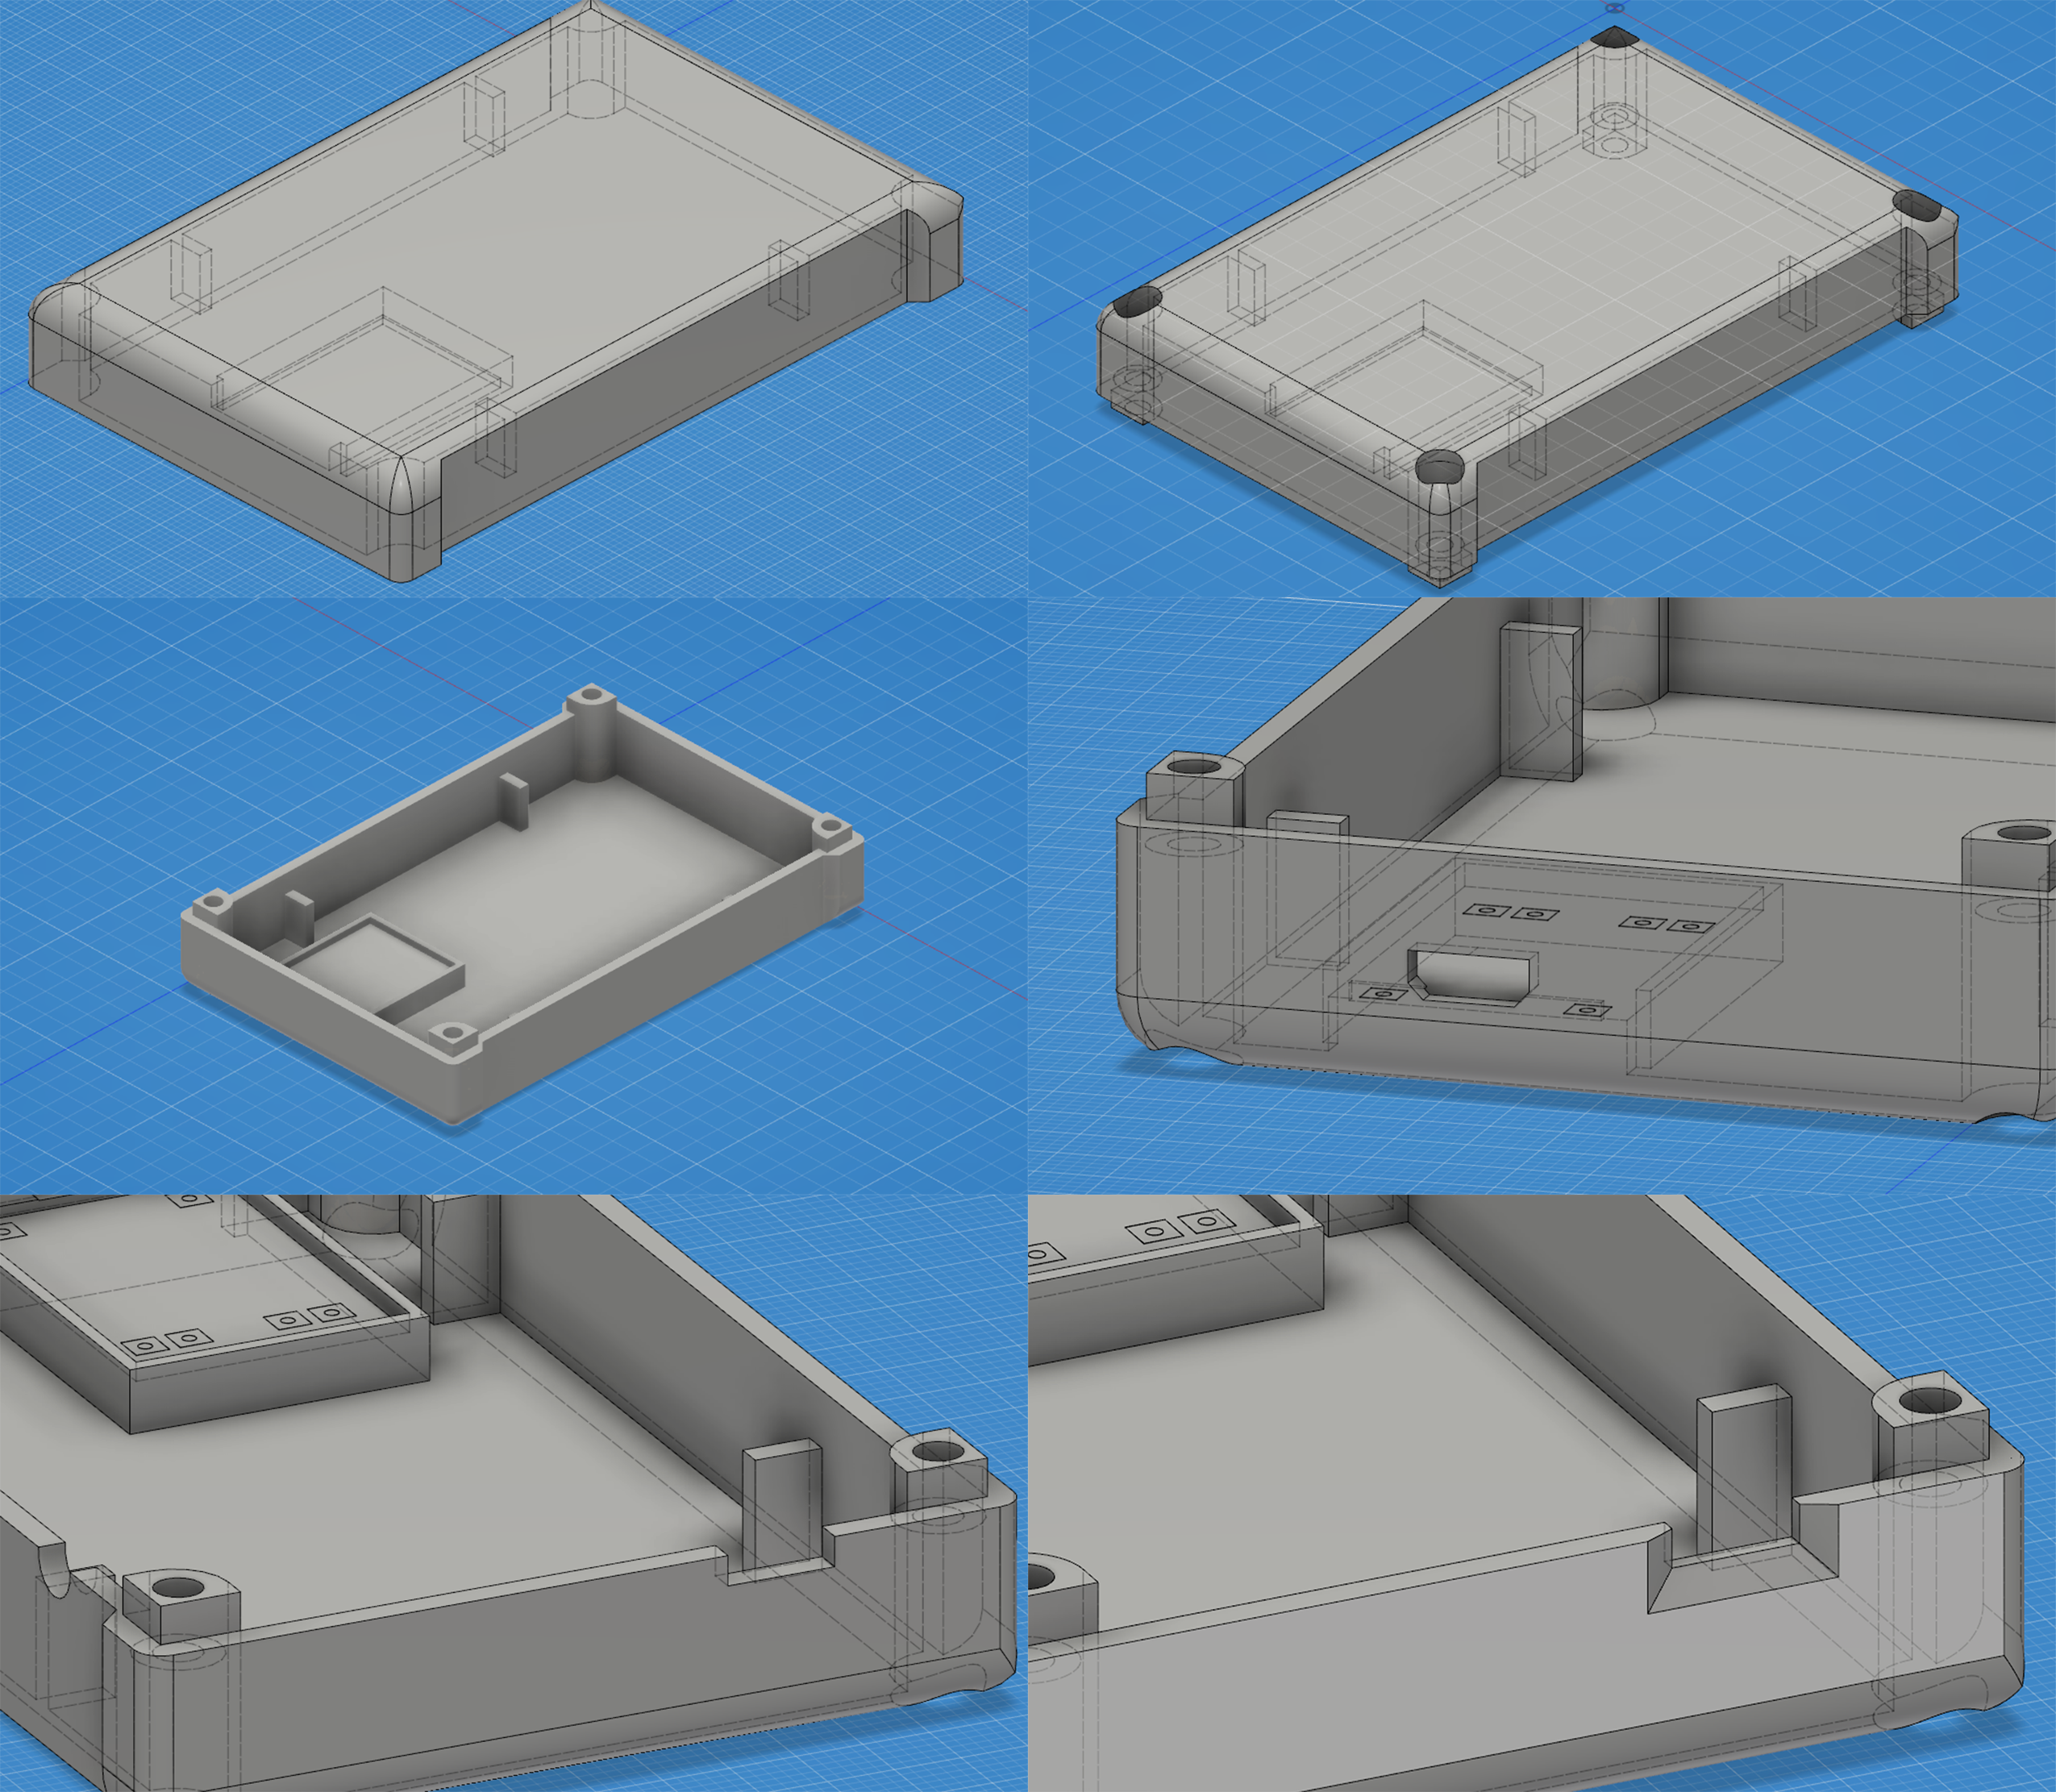
\includegraphics[width=0.7\linewidth]{armazon09.png}
	\caption{Proceso del diseño del molde inferior parte 2}
\end{figure}

\begin{figure}[H]
	\centering
	\includegraphics[width=0.8\linewidth]{armazon10.png}
	\caption{Diseño del molde inferior finalizado}
\end{figure}

\begin{figure}[H]
	\centering
	\includegraphics[width=0.8\linewidth]{armazon11.png}
	\caption{Diseño del final del armazón}
\end{figure}

\par \noindent
Una vez diseñado el molde superior e inferior procedemos a realizar la impresión 3D de los mismos y el ensamblaje final.

